\chapter{Planificación del Proyecto} \label{requisitos}

\section{Propósito}

En este capítulo se llevará a cabo la planificación de las diferentes etapas que compondrán el desarrollo del proyecto. Para la realización de esta planificación de la manera más profesional y cercana a la realidad del desarrollo software moderno, se van a aplicar algunos conceptos propios de \textbf{Scrum} \cite{scrum} como metodología ágil \ref{fig:scrum-logo} .
\begin{figure}[H]
    \centering
    
\includegraphics[width=0.5\textwidth]{fotos/scrum.png}
    \caption{Metodología ágil Scrum\textbf{}.}
    \label{fig:scrum-logo}
\end{figure}
Tras estudiar los distintos principios en los que se basa Scrum se han identificado varios elementos clave entre los que destacan: la necesidad de participación activa por parte del cliente y la existencia tanto de un equipo de desarrollo como de profesionales con roles específicos tales como \textit{Scrum Master} y \textit{Product Owner}. Sin embargo, en el contexto de la realización de un Trabajo de Fin de Grado, estas condiciones resultan inviables debido al carácter individual del mismo. No se cuenta ni con un equipo de desarrollo, ni existe ningún integrante con capacidad para realizar dichos roles. Además la participación del cliente es totalmente inexistente.

A pesar de estas limitaciones, y con el objetivo de que el proyecto tenga un desarrollo lo más profesional y realista posible, se adaptarán varios elementos presentes en la metodología Scrum en la planificación. Estos elementos a considerar van a ser:

\begin{itemize}
    \item \textbf{Iteraciones}: El proyecto se desarrollará a través de ciclos iterativos en los que se encapsulan bloques importantes de funcionalidad, se asemejará en concepto a los Sprint de Scrum pero sin la necesidad de terminar siempre con un objeto minimamente viable evaluado por el cliente.
    \item \textbf{Historias de Usuario}: Se usarán las historias de usuario para describir funcionalidades específicas del sistema, desde la perspectiva del usuario final.
    \item \textbf{Incremento de Funcionalidad}: En cada iteración se conseguirá un incremento funcional del proyecto, que podrá ser revisado y mejorado en las siguientes iteraciones.
    \item \textbf{Adaptabilidad}: La planificación de cada iteración podrá ser modificada en función del progreso realizado y las necesidades detectadas.
    \item \textbf{Revisión}: Al final de cada iteración se realizará un análisis para idenitifcar que elementos se pueden mejorar y cuáles se están haciendo bien.
\end{itemize}

Para mayor referencia, se puede consultar la guía oficial de Scrum\cite{scrumguide2020}. 
Una vez establecidas las bases que van a constituir la planificación del proyecto, se va a proceder a realizar un análisis de la velocidad de desarrollo.

\section{Cálculo de la Velocidad de Desarrollo}
\label{sec:velocidad-desarrollo}
Para realizar la estimación de la velocidad de desarrollo de las distintas funcionalidades del sistema, vamos primero a analizar las condiciones iniciales:

\begin{itemize}
    \item Contamos con un \textbf{único desarrollador}.
    \item Se dedicarán \textbf{2.5 horas efectivas} al día al proyecto.
    \item Cada iteración tendrá una duración de \textbf{3 semanas}, siendo un total de \textbf{4 iteraciones}.
    \item Se trabajará un total de 5 días efectivos a la semana al proyecto.
\end{itemize}

A continuación, estimaremos el tiempo medio de desarrollo de un \textbf{Punto de Historia de Usuario}, que será la unidad de medida del esfuerzo requerido para cada tarea. 

Inicialmente, asignaremos un total de 3 horas de trabajo a cada Punto de Historia de Usuario. Con esto establecido, el cálculo de las horas efectivas por iteración es el siguiente:
\begin{equation*}
    \text{Horas efectivas por iteración} = 3 \text{ semanas} \times 5 \text{ días por semana} \times 3 \text{ horas diarias}
\end{equation*}
\begin{equation*}
    = 3 \times 5 \times 3 = 45 \text{ horas por iteración}
\end{equation*}

Si consideramos que cada Punto de Historia de Usuario requiere \textbf{3 horas de trabajo}, entonces la cantidad de Puntos de Historia de Usuario que pueden desarrollarse en una iteración será:

\begin{equation*}
    \frac{45 \text{ horas}}{2,5 \text{ horas por punto}} = 18 \text{ puntos de historia por iteración}    
\end{equation*}


Por tanto, de manera inicial tomaremos como referencia que en cada iteración se podrán desarrollar \textbf{18 Puntos de Historia de Usuario}.

Este cálculo podrá verse modificado en función del resultado real de cada iteración, por lo que será revisado y ajustado si es necesario.


Finalmente se muestra una tabla resumen con los valores más relevantes de esta sección.
\begin{table}[H]
    \centering
    \renewcommand{\arraystretch}{1.3}
    \begin{tabular}{|l|c|}
        \hline
        \rowcolor[HTML]{D3D3D3} 
        \textbf{Parámetro} & \textbf{Valor} \\ \hline
        Desarrolladores & 1 \\ \hline
        Horas efectivas diarias & 2.5 horas \\ \hline
        Días efectivos por semana & 5 días \\ \hline
        Duración de cada iteración & 3 semanas (21 días) \\ \hline
        Horas efectivas por iteración & 45 horas \\ \hline
        Tiempo estimado por Punto de Historia & 2,5 horas \\ \hline
        Velocidad total por iteración & 18 PHUs \\ \hline
    \end{tabular}
    \caption{Resumen de parámetros para la estimación de velocidad de desarrollo}
    \label{tab:estimacion_velocidad}
\end{table}


\section{Listado de historias de usuario}
A continuación, se muestra una lista con las historias de usuario que describirán la funcionalidad del proyecto, a cada una se le ha asignado una serie de puntos de historia de usurio (PHU) en función de su aparente complejidad.
\newpage

\renewcommand{\arraystretch}{1.3}
\begin{longtable}{|c|p{12cm}|c|}
    \hline
    \textbf{Código} & \textbf{Título} & \textbf{PHU} \\
    \hline \hline
    HU01 & Como usuario buscador, quiero poder darme de alta en la aplicación para encontrar una comunidad a la que unirme. & 3 \\
    \hline
    HU02 & Como usuario buscador, quiero poder darme de baja de la aplicación, eliminando todos mis datos. & 2 \\
    \hline
    HU03 & Como usuario buscador, quiero poder configurar mis gustos y preferencias para recibir recomendaciones de comunidades afines. & 2 \\
    \hline
    HU04 & Como usuario buscador, quiero que el sistema me recomiende comunidades en función del grado de afinidad que compartimos. & 3 \\
    \hline
    HU05 & Como usuario buscador, quiero poder dar me gusta a los pisos que me interesan para guardarlos en una colección. & 1 \\
    \hline
    HU06 & Como usuario buscador, quiero poder consultar todas las comunidades a las que les he dado me gusta. & 2 \\
    \hline
    HU07 & Como usuario buscador, quiero visualizar en detalle la información de una comunidad (integrantes, preferencias, imágenes, localización y precio). & 2 \\
    \hline
    HU08 & Como usuario buscador, quiero poder solicitar unirme a una comunidad que me interese, para pasar a formar parte de ella. & 3 \\
    \hline
    HU09 & Como usuario buscador, quiero recibir notificaciones cuando acepten o rechacen mi solicitud de unión a una comunidad. & 1 \\
    \hline
    HU10 & Como usuario buscador, quiero establecer filtros en la búsqueda de vivienda (localización, número de habitaciones, precio y espacio). & 2 \\
    \hline
    HU11 & Como usuario buscador, quiero que el sistema me muestre las comunidades ordenadas en función del grado de afinidad. & 2 \\
    \hline
    HU12 & Como usuario ofertante, quiero poder darme de alta en el sistema para buscar integrantes con los que compartir mi comunidad. & 3 \\
    \hline
    HU13 & Como usuario ofertante, quiero poder darme de baja en el sistema, eliminando todos mis datos contenidos. & 1 \\
    \hline
    HU14 & Como usuario ofertante, quiero poder dar de alta una comunidad, introduciendo nombre, integrantes, localización, precio, criterios de afinidad y fotos. & 3 \\
    \hline
    HU15 & Como usuario ofertante, quiero consultar el perfil de cada usuario que envía una solicitud de unión, para conocer sus preferencias y el grado de afinidad. & 2 \\
    \hline
    HU16 & Como usuario ofertante, quiero poder aceptar o rechazar usuarios que solicitan unirse a mi comunidad. & 2 \\
    \hline
    HU17 & Como usuario ofertante, quiero recibir una notificación cuando un usuario solicite unirse a mi comunidad. & 1 \\ 
    \hline
    HU18 & Como usuario ofertante, quiero poder modificar la información de mi comunidad para mantenerla actualizada. & 2 \\
    \hline
    HU19 & Como usuario ofertante, quiero poder eliminar una comunidad, borrando toda la información contenida en el sistema. & 1 \\
    \hline
    HU20 & Como usuario ofertante, quiero poder eliminar un usuario de mi comunidad en caso de incumplimiento de normas. & 1 \\
    \hline
    HU21 & Como usuario buscador u ofertante, quiero poder consultar el calendario de tareas y actividades del piso. & 3 \\
    \hline
    HU22 & Como usuario buscador u ofertante, quiero visualizar en el calendario las tareas o actividades previstas en un día concreto, con detalles como hora, descripción y participantes. & 3 \\
    \hline
    HU23 & Como usuario buscador u ofertante, quiero que tanto las actividades como las tareas se añadan al calendario automáticamente para que mis compañeros las vean. & 2 \\
    \hline
    HU24 & Como usuario buscador u ofertante, quiero poder añadir eventos al calendario para que mis compañeros puedan consultarlos fácilmente. & 2 \\
    \hline
    HU25 & Como usuario buscador u ofertante, quiero poder registrar tareas a realizar mediante un formulario donde especifique dificultad, tiempo para realizarla y descripción. & 3 \\
    \hline
    HU26 & Como usuario buscador u ofertante, quiero poder registrar actividades a realizar mediante un formulario indicando lugar, fecha, hora y descripción. & 3 \\
    \hline
    HU27 & Como usuario buscador u ofertante, quiero recibir una notificación cuando se asignen las tareas semanales. & 2 \\
    \hline
    HU28 & Como usuario buscador u ofertante, quiero distribuirme las tareas libremente a lo largo de la semana según mis necesidades. & 3 \\
    \hline
    HU29 & Como usuario buscador u ofertante, quiero recibir una notificación con una hora de antelación antes de que termine el plazo de una tarea. & 2 \\
    \hline
    HU30 & Como usuario buscador u ofertante, quiero que al final de la semana se genere un resumen con las tareas completadas por cada integrante. & 2 \\
    \hline
    HU31 & Como usuario buscador u ofertante, quiero que si no distribuyo manualmente mis tareas en un tiempo límite, el sistema las asigne automáticamente. & 2 \\
    \hline
    HU32 & Como usuario buscador u ofertante, quiero poder reorganizar las tareas asignadas para poder cumplir con contratiempos personales. & 2 \\
    \hline
    HU33 & Como usuario buscador u ofertante, quiero que la asignación de tareas semanales sea cíclica, para que todos los integrantes hagan todas las tareas equitativamente. & 2 \\
    \hline
    HU34 & Como usuario buscador u ofertante, quiero que los usuarios que no realicen sus tareas sean penalizados, reasignándoselas con un plazo de tiempo limitado. & 2 \\
    \hline
\end{longtable}

\section{Descripción de las iteraciones}

El desarrollo del proyecto se estructurará en cuatro iteraciones, permitiendo descomponer el trabajo en grandes grupos de tareas bien definidos. En cada iteración se llevará a cabo la realización de un bloque completo de funcionalidad de manera que se vaya iterando hacia un producto más completo.

\subsection{Duración y Esfuerzo}
Para establecer las iteraciones del proyecto, se ha planteado un desarrollo basado en cuatro iteraciones de una duración de tres semanas cada una. De este modo, el esfuerzo total requerido por el proyecto se representa con \textbf{72 Puntos de Historia de Usuario (PHUs)}, asignando una velocidad de desarrollo previamente calculada de \textbf{18 PHUs} por iteración.

\subsection{Distribución de Funcionalidades}
Dado que en cada iteración se completarán 18 PHUs, en la planificación se ha buscado priorizar aquellas historias de usuario de mayor complejidad y que aportan más valor al sistema en las primeras iteraciones. Este enfoque garantiza que, en caso de retrasos, haya tiempo suficiente para asegurar una funcionalidad básica.

\begin{itemize}
    \item \textbf{Iteración 0} \textit{(Documentación e investigación)}: Esta iteración, visible en el diagrama de Gantt  \ref{fig:gantt0}, abarca todo el proceso previo de documentación realizado hasta el momento, así como la investigación y el aprendizaje de las tecnologías necesarias para el desarrollo, este proceso de documentación pese a que se seguirá realizando en las siguientes iteraciones en esta ha tenido un papel clave por lo que no seguirá la misma estructura ni temporal ni de historias de usuario que las demás.

    \item \textbf{Iteración 1} \textit{(Registro de usuarios y configuración de comunidades, Diagrama de Gantt  \ref{fig:gantt1})}:
    \begin{itemize}
        \item Objetivo: Implementar la lógica básica del sistema, permitiendo el registro de usuarios buscadores como ofertantes, la configuración de preferencias en su perfil y la creación de comunidades. Se continua con la documentación del proyecto.
        \item Historias de usuario: HU01, HU02, HU03, HU12, HU13, HU14, HU18, HU19, HU20.
        \item Puntos de Historia asignados: 18 PHUs.
    \end{itemize}
    
    \item \textbf{Iteración 2} \textit{(Búsqueda de piso y algoritmo de recomendación, Diagrama de Gantt  \ref{fig:gantt2})}:
    \begin{itemize}
        \item Objetivo: Implementar la búsqueda de pisos mediante filtros, las solicitudes de unión a comunidades y el algoritmo de recomendación basado en afinidad. Se continua con la documentación del proyecto.
        \item Historias de usuario: HU04, HU07, HU08, HU09, HU10, HU11, HU15, HU16, HU17.
        \item Puntos de Historia asignados: 18 PHUs.
    \end{itemize}
    
    \item \textbf{Iteración 3} \textit{(Gestión de tareas y calendario, Diagrama de Gantt \ref{fig:gantt3})}:
    \begin{itemize}
        \item Objetivo: Desarrollar la lógica relacionada con la gestión de tareas y actividades, desde su creación, modificación y asignación, incluyendo el calendario compartido. Se continua con la documentación del proyecto.
        \item Historias de usuario: HU21, HU22, HU23, HU24, HU25, HU26, HU33.
        \item Puntos de Historia asignados: 18 PHUs.
    \end{itemize}
    
    \item \textbf{Iteración 4} \textit{(Funcionalidades adicionales, Diagrama de Gantt  \ref{fig:gantt4})}:
    \begin{itemize}
        \item Objetivo: Incorporar funcionalidades complementarias para mejorar la experiencia del usuario. Se continua con la documentación del proyecto.
        \item Historias de usuario: HU05, HU06, HU27, HU28, HU29, HU30, HU31, HU32, HU34.
        \item Puntos de Historia asignados: 18 PHUs.
    \end{itemize}
\end{itemize}

\section{Diagrama de Gantt}

Para poder visualizar de forma esquematizada el contenido de las distintas iteraciones que va a tener el proyecto se ha realizado un diagrama de Gantt.

En el diagrama podremos analizar diversas características clave, como la duración de cada iteración, el tiempo requerido para completar cada historia de usuario y el avance progresivo del proyecto.

\begin{figure}[H]
    \centering
    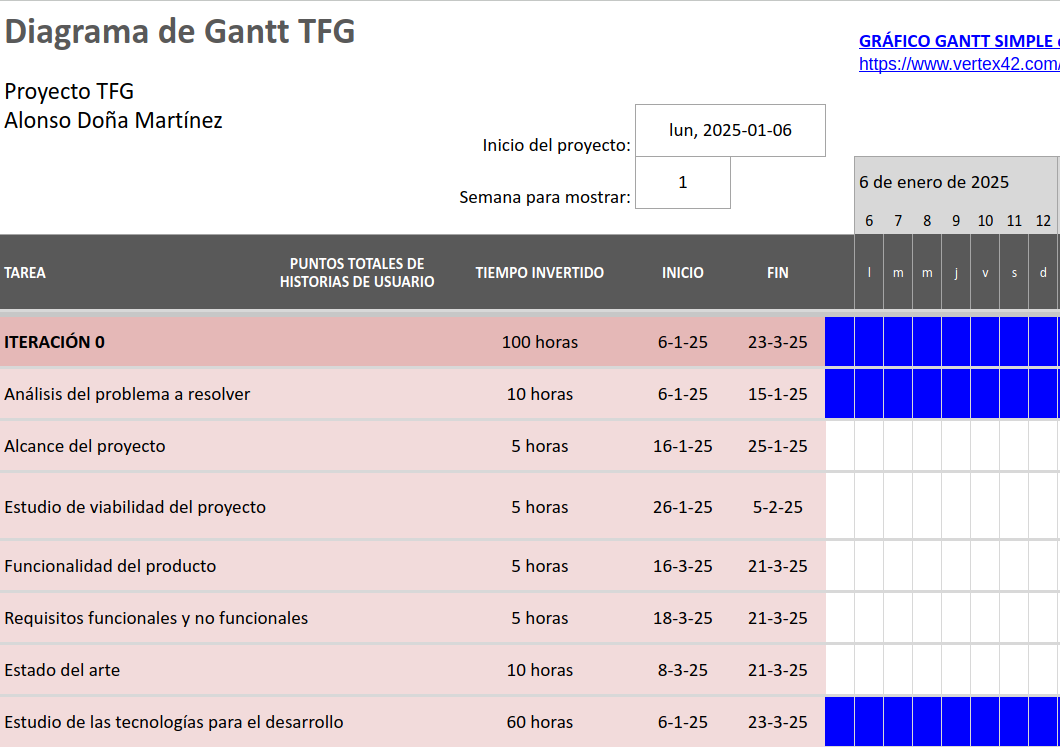
\includegraphics[width=1\textwidth]{fotos/iter0.png}
    \caption{Diagrama de Gantt iteración 0\textbf{}.}
    \label{fig:gantt0}
\end{figure}
\begin{figure}[H]
    \centering
    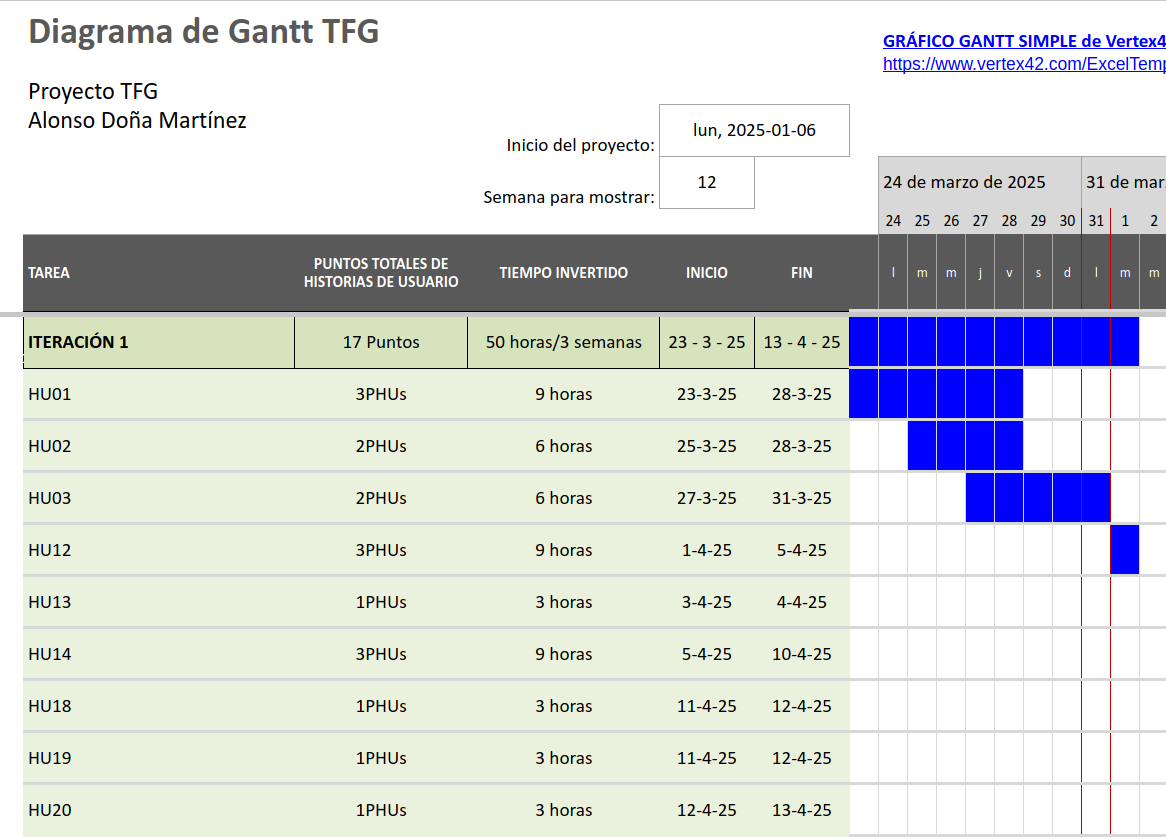
\includegraphics[width=1\textwidth]{fotos/iter1.png}
    \caption{Diagrama de Gantt iteración 1\textbf{}.}
    \label{fig:gantt1}
\end{figure}
\begin{figure}[H]
    \centering
    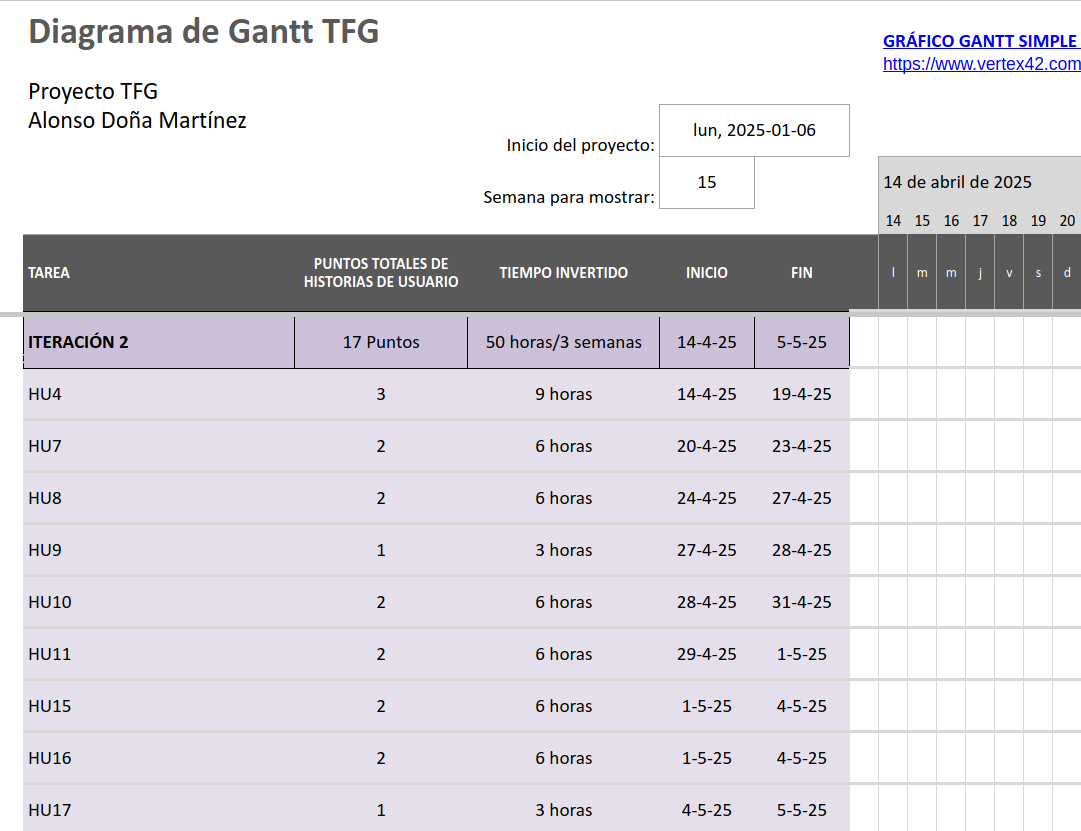
\includegraphics[width=1\textwidth]{fotos/iter2.png}
    \caption{Diagrama de Gantt iteración 2\textbf{}.}
    \label{fig:gantt2}
\end{figure}
\begin{figure}[H]
    \centering
    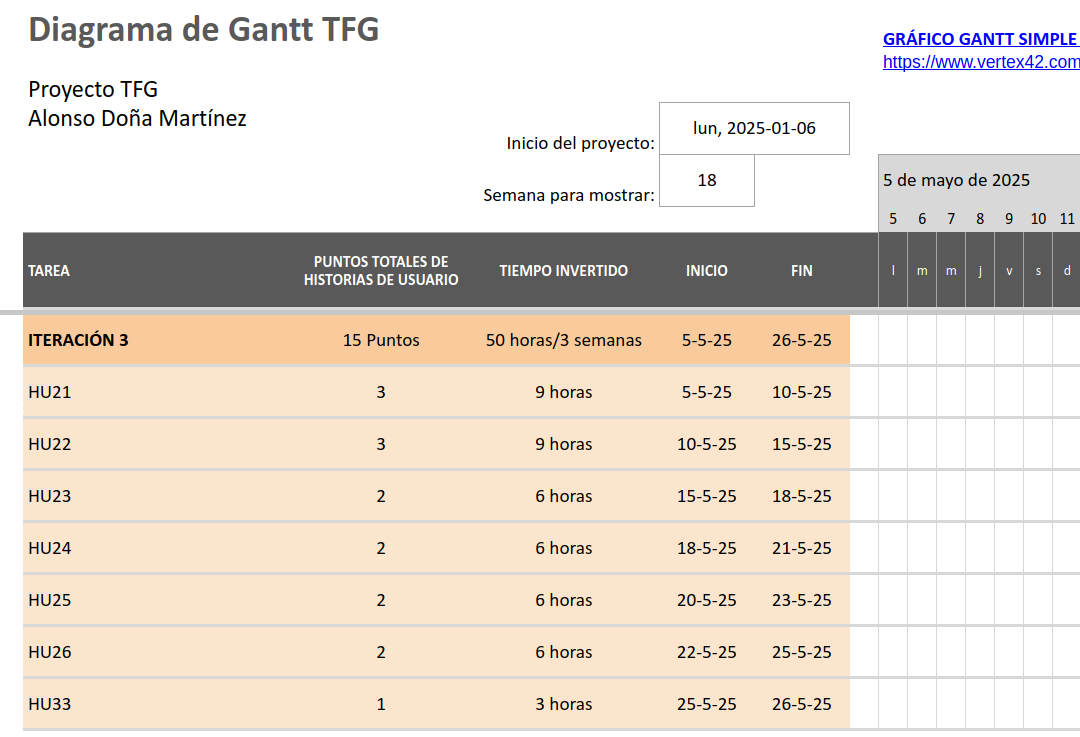
\includegraphics[width=1\textwidth]{fotos/iter3.png}
    \caption{Diagrama de Gantt iteración 3\textbf{}.}
    \label{fig:gantt3}
\end{figure}
\begin{figure}[H]
    \centering
    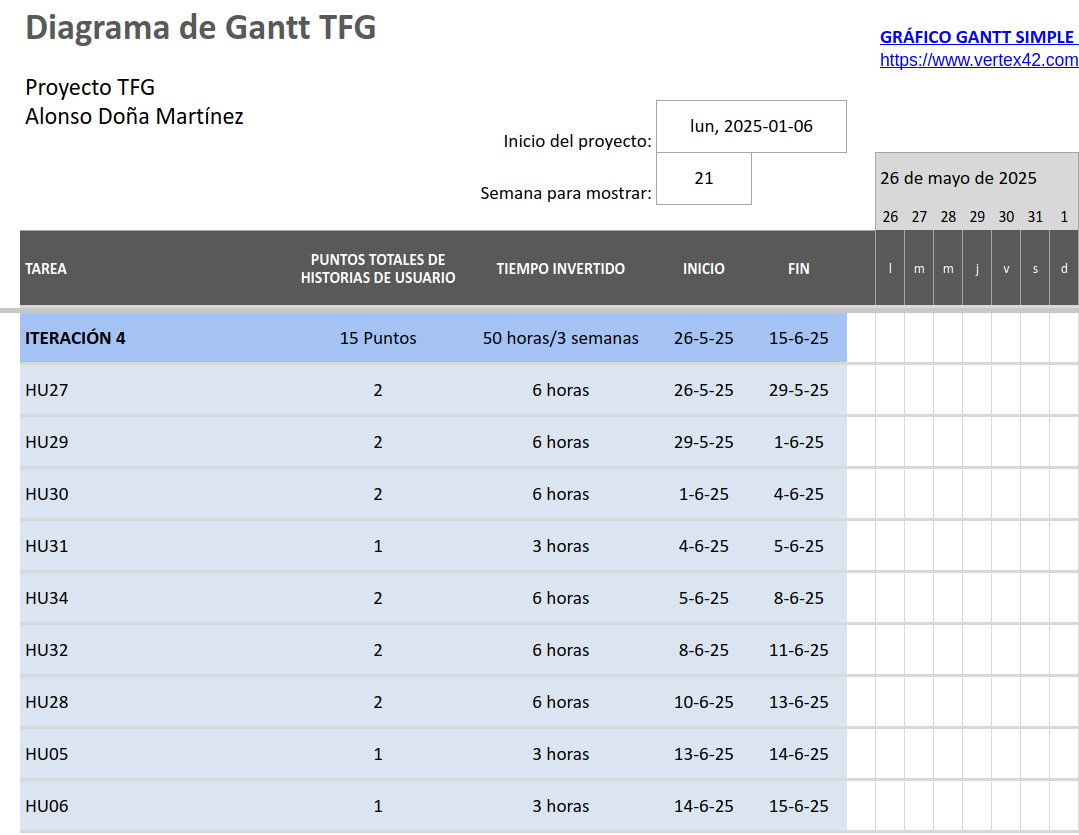
\includegraphics[width=1\textwidth, height=10cm]{fotos/iter4.png}
    \caption{Diagrama de Gantt iteración 4\textbf{}.}
    \label{fig:gantt4}
\end{figure}
\section{Estimación de costes}
Para el cálculo de la estimación de costes del proyecto vamos a desglosar el presupuesto en varias secciones.

\subsection{Costes de Herramientas Utilizadas}
El desarrollo del proyecto se ha realizado utilizando un ordenador portátil HP Pavilion adquirido en el año 2021, por un coste de \textbf{782 euros}. Se ha decidido amortizar este equipo con una tasa del 20\% por año, lo que resulta en un coste total de:

\begin{equation*}
    \text{Coste anual} = 782 \times 0.20 = 156.4 \, \text{euros}
\end{equation*}
\begin{equation*}
    \text{Resto total} = 156.4 \times 4 = 625.6 \, \text{euros}
\end{equation*}
Por tanto, si restamos este coste al valor total del equipo, obtenemos:
\begin{equation*}
     \text{Coste final: } 782 - 625.6 = 156.4 \, \text{euros}
\end{equation*}

\subsection{Coste de Desarrollo}
Para calcular el coste de desarrollo, utilizamos la velocidad estimada en el capítulo \ref{sec:velocidad-desarrollo}. En él se determinó que cada iteración contará con un total de 45 horas de trabajo, contando con un total de 4 iteraciones, además de la fase de investigación y aprendizaje previa a la que se le ha asignado un total de 100 horas.  

El total de horas dedicadas será:

\begin{equation*}
    4 \times 45 + 100 = 280 \text{ horas}
\end{equation*}

Si consideramos que el sueldo medio anual de un ingeniero de software en España en 2025, es de 32,850 euros, según \href{https://www.glassdoor.es/Sueldos/ingeniero-de-software-sueldo-SRCH_KO0,21.htm}{Glassdoor}, y suponiendo una jornada laboral de 1,800 horas anuales y unos 2,190 euros netos al mes, el coste por hora se obtiene de la siguiente forma:

\begin{equation*}
    \text{Coste por hora} = \frac{2190 \, \text{euros}}{40 \, \text{horas/semana} \times 4 \, \text{semanas/mes}} = \frac{2190}{160} = 13.68 \, \text{euros/hora}
\end{equation*}

A continuación, si se han invertido aproximadamente 280 horas en el desarrollo, el coste total de desarrollo sería:

\begin{equation*}
    \text{Coste de desarrollo} = 280 \, \text{horas} \times 13.68 \, \text{euros/hora} = 3830,4 \, \text{ euros}
\end{equation*}

Así, el coste total de desarrollo, basado en las horas dedicadas y el coste por hora de un ingeniero de software, sería de 3830,4 euros.



\subsection{Costes de Infraestructura}
Se ha optado por el uso de tecnologías de código libre y herramientas gratuitas, lo que permite que todos los costes asociados a la infraestructura de desarrollo sean nulos.

\subsection{Coste de Mantenimiento}
El mantenimiento de la aplicación incluirá la corrección de errores y la implementación de nuevas funcionalidades. Se estima que representará el 25\% del total de horas dedicadas al desarrollo del proyecto.

Por tanto, el número de horas de mantenimiento se calcula como:

\begin{equation*}
    Horas_{\text{mantenimiento}} = 0.25 \times 280\text{ (horas totales dedicadas al desarrollo)} = 70 \text{ horas}
\end{equation*}

El coste total de mantenimiento será:

\begin{equation*}
    Coste_{\text{mantenimiento}} = 70 \times 13.68 = 957,6 \text{ euros}
\end{equation*}
\subsection{Resumen de Costes}
En la Tabla \ref{tab:costes} se presentan los costes asociados al desarrollo del proyecto. Dichos costes suman un total final de 5132,81\euro

\begin{table}[h]
    \centering
    \renewcommand{\arraystretch}{1.3}
    \begin{tabular}{|l|c|}
        \hline
        \textbf{Concepto} & \textbf{Coste (euros)} \\
        \hline
        Amortización del portátil & 156.4\euro \\
        Coste de desarrollo & \( 3830,4\euro \) \\
        Coste de infraestructura & 0\euro \\
        Coste de mantenimiento & \( 957,6\euro \) \\
        \hline
        \textbf{Total} & \( 4944,4 \) \\
        \hline
    \end{tabular}
    \caption{Resumen de costes del proyecto}
    \label{tab:costes}
\end{table}

